\documentclass[a4paper,10pt]{report}
\usepackage[utf8x]{inputenc}
\usepackage[T1]{fontenc}
\usepackage[french]{babel} 
\usepackage{lmodern} % Pour changer le pack de police
\usepackage{makeidx}
\usepackage{graphicx}
\graphicspath{{figures/}}
\usepackage[margin=3cm]{geometry}
\usepackage{array}

\title{Projet 3A\\Analyse d'imagerie polarimétrique}
\author{\textsc{Guinaudeau} Alexandre\\
	\and 
	\textsc{Hulot} Pierre
	\and 
	\textsc{Dejoie} Etienne	
	}
\date{\today}
\makeindex
\begin{document}

\maketitle

\begin{abstract}
Le résumé (abstract en anglais) de mon article.
\end{abstract}

\section*{Introduction}


Aujourd'hui, le dépistage du cancer du col de l'utérus est effectué à l'\oe il nu. Si la patiente est effectivement atteinte d'un cancer, un échantillon (appelé conisation) est prélevé, et un spécialiste découpe l'échantillon pour déterminer les zones atteintes. 
\emph{ADM polar} cherche à détecter les cellules cancéreuses à partir d'imagerie polarimétrique. 
L'idée à terme serait de concevoir un outil qui permette de détecter les zones effectivement atteintes \emph{in vivo}, pour ainsi mieux délimiter la zone à prélever et réduire les risques de prélèvement pour les patientes saines.


\emph{ADM polar} fait analyser ces échantillons par un spécialiste, pour déterminer l'état (sain, malade, bénin...) des cellules le long de coupes.
Puis, après avoir pris plusieurs images dans des configurations de polarisation différentes, \emph{ADM polar} reconstitue la matrice de Müller de l'échantillon, un ensemble de 16 images qui représentent l'état de polarisation.
Il reste alors à déterminer la corrélation entre les valeurs dans la matrice de Müller d'une cellule et son diagnostique.


Dans le cadre du projet de 3e année, nous avons souhaité appliquer les connaissances théoriques apprises en cours à des données réelles. Nous avons donc rejoint le projet d'\emph{ADM polar}, dans le but de détecter les cellules cancéreuses, à partir des images polarimétriques fournies par \emph{ADM polar}.


La première étape a été la visualisation des données, pour mieux savoir quels modèles d'apprentissage seraient les plus susceptibles de porter leurs fruits. Puis, nous avons cherché à réduire la dimension du problème en sélectionnant ls paramètres les plus discriminants dans la classification des cellules. Enfin, nous avons testé différents modèles de classification et mesuré leur performance en termes de précision et de coût de calcul.

\chapter{Contexte}
\section{ADM Polar, contexte du projet}
\section{Présentation des données}
Pour ce projet nous disposions d'un jeu de données de $163 000$ pixels répartis sur 17 images différentes. Pour chaque pixel nous avions les 16 éléments de la matrice de Müller, leur position, leur diagnostic, et l'image correspondante.
Ces Pixels sont répartis en $4/5$ de sains et $1/5$ de malades. L'affichage des pixels nous montre que dans chaque image, les pixels sont répartis en zones au diagnostic identique. Sur les $17$ images, $11$ possèdent que des zones saines, une a une zone saine et une zone malade et les $5$ dernières ont que des zones malades. Le nombre d'images étant assez limité il n'a été facile de trouver des points communs aux pixels sain et aux pixels malades.


mettre les images ici. (toutes?)

\subsection{la Matrice de Müller}
\index{Matrice de Muller}
Les données sont obtenues par polarisation de la lumière. De la lumière polarisée est envoyée sur l'échantillon, réfléchi par celui ci est analysé ensuite.
La matrice de Müller est obtenue à partir de l'analyse de la polarisation de la lumière réfléchie. Le postulat du laboratoire sur lequel repose tout le traitement des données est que les cellules saines et malades polarisent différemment la lumière. Cela implique qu'il est possible de reconnaître une cellule malade par la polarisation de la lumière réfléchie.
Le PICM se bases pour cela d'observations de relation entre les images polarisées et le diagnostic. 
La polarisation génère 16 images par échantillon. On associe alors à chaque pixel une matrice $4x4$ appelée matrice de Müller. Dans cette matrice, la première ligne et la première colonne représentent l'intensité du signal, ces éléments influent peu sur le diagnostic mais ont des valeur élevés, ils introduisent beaucoup de biais et de sur-apprentissage. Nous avons donc décidé de ne pas les prendre en compte. Les éléments diagonaux sont normalement censé être les plus significatifs mais les reflets introduisent beaucoup de bruit rendant ces données difficilement utilisables. Il reste 6 éléments dans la matrices sur lesquels nous allons nous concentrer. 

\subsection{Le Clustering}
La disposition des données n'étant pas facilement exploitable directement il fallait réduire la complexité du problème, par exemple en limitant le nombre de données. Nous avons ainsi décidé de clustériser les données de chaque image afin d'en avoir beaucoup moins, mais plus significatives. La position du pixel dans l'image n'a pas été prise en compte, même si les zones résultantes sont proches. La clustérisation à été faite par un algorithme de type KNN (k plus proches voisins) sur les $6$ éléments significatifs de la matrice de Müller. Les diagnostics étant propres à chaque image (une seule image avec un diagnostic non uniforme), chaque cluster est associé à un diagnostic. 

La méthode de clustering utilisé consiste en :
\begin{itemize}
\item choisir k, le nombre de clusters
\item regrouper les pixels de l'image selon ces k clusters (par $KNN$)
\item calculer l'erreur totale commise (somme des distances au centre du cluster)
\item recommencer avec un k plus grand si l'erreur est trop grande
\end{itemize}

Cette méthode nous a permis de passer de $163 000$ points à $52$ plus significatifs. Elle nous a aussi permis de mieux comprendre la répartition des points. Le clustering a surtout un apport au niveau de la compréhension des données. Il pourrait avoir un impact (en tant que tel) sur les résultats, mais son but a été surtout de mieux comprendre la disposition des données pour pouvoir apprendre dessus.
\chapter{Le traitement des données}

\section{Prétraitement des données}
Le Prétraitement de données est l'étape essentielle qui précède l'apprentissage. Elle est la clé de celui ci, un bon prétraitement permet d'éliminer le bruit et présente les données sous un angle facilement exploitable. C'est là que se situe tout l'enjeu d'un classifieur Big Data ainsi que le travail d'un data analyst, les méthodes d'apprentissage étant préexistantes.  

Les différents types de prétraitements que l'on peut faire avant de traiter les données
\section{Les différentes approches de traitement des données}

\subsection{Réduction de dimension}
\subsubsection{PCA}
\paragraph{rappel de la méthode }
L'Analyse en Composantes Principales (ou PCA) consiste à essayer de représenter les données dans un espace de plus petites dimensions. Les vecteurs directeurs du nouvel espace maximise la variance entre les données. Nous présentons ici les résultats pour la dimension 2.
\paragraph{prétraitement utilisé}
Nous effectuons cette PCA sur les centres des clusters préalablement présentés (cf 1.1.1). Les centres des clusters représentent de manière fidèle l'ensemble des points qu'il rassemble. Chaque cluster est représenté par un vecteur d'éléments de la matrice de Müller. Tous les éléments de Müller sont gardés à l’exception de la première ligne et première colonne qui ne sont pas a priori pertinentes (d'après les informations des physiciens)
\begin{figure}
  \caption{centre des clusters avant transformation}
  \centering
  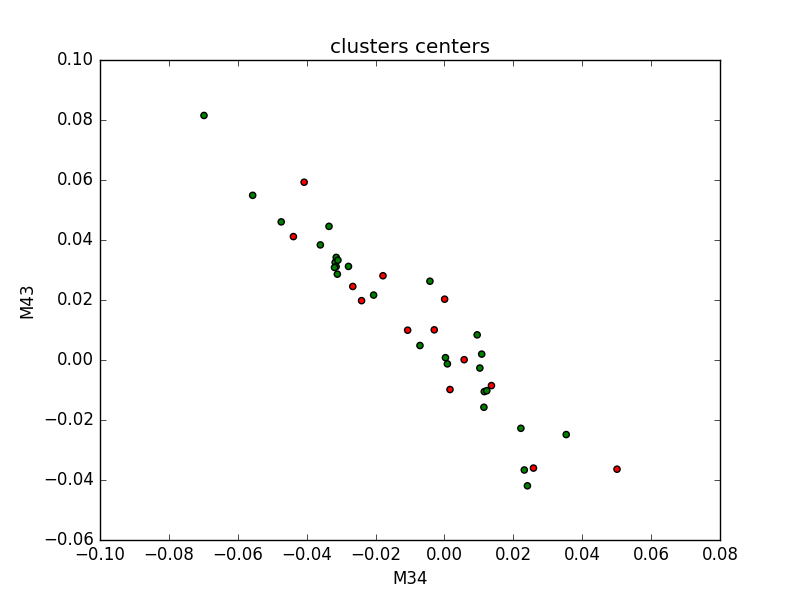
\includegraphics[width=10cm]{PCA_0.png}
\end{figure}
\begin{figure}
  \caption{centre des clusters après transformation}
  \centering
  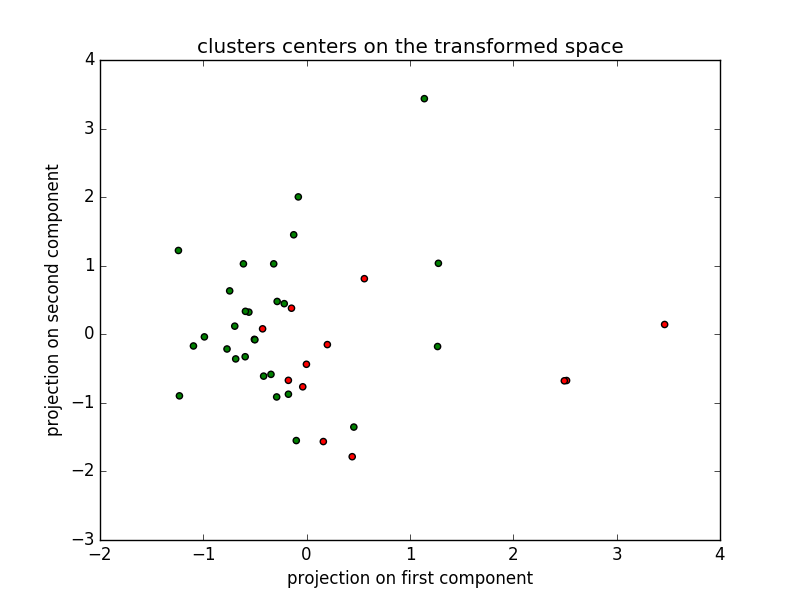
\includegraphics[width=10cm]{PCA_1.png}
\end{figure}
\begin{figure}
  \caption{Part de variance expliquée}
  \centering
  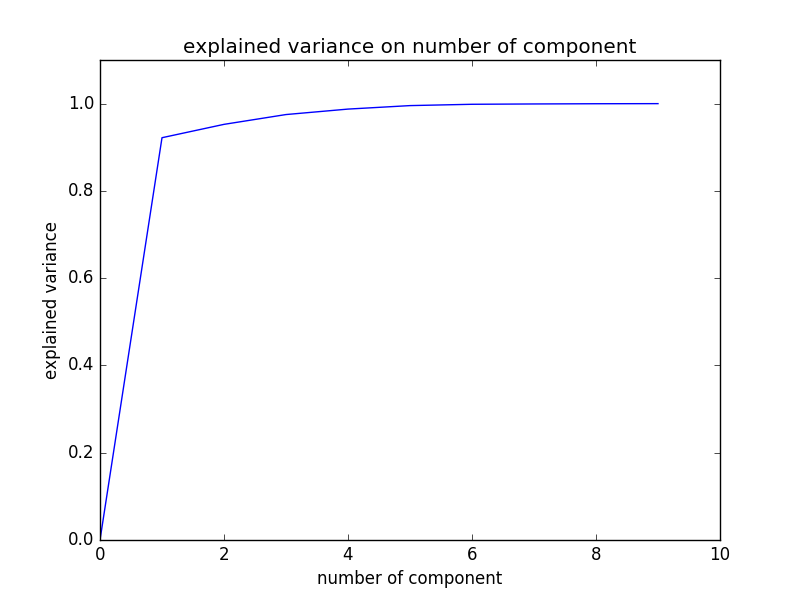
\includegraphics[width=10cm]{PCA_3.png}
\end{figure}
\begin{figure}
  \caption{analyse de la composante principale}
  \centering
  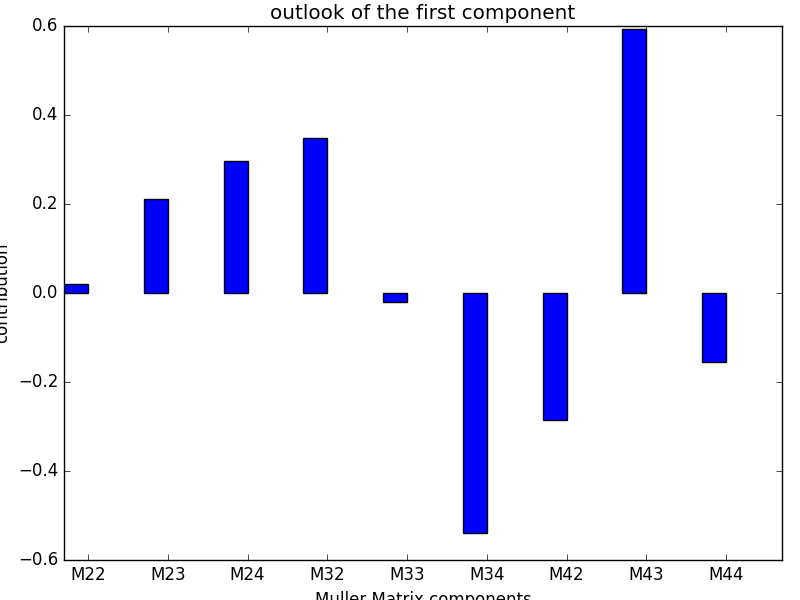
\includegraphics[width=10cm]{PCA_2.png}
\end{figure}

\paragraph{résultats}
La réduction de dimension par PCA semble efficace. La composante principale explique 90\% de la variance (fig 2.3). 
De l'analyse de la première composante (fig 2.4) ressort deux effets principaux :
- La petite contribution des éléments diagonaux de la matrice de Müller
- Le rôle prépondérant de M34 et M43

On remarque une certaine anti-corrélation des éléments de la matrice de Müller. Le poids de M43 est proche de l'opposé de celui de M34. Le poids de M42 est également proche de l'opposé de celui de M24. Cette observation n'est par contre pas vérifiée pour M23 et M32 qui semblent corrélés.
\paragraph{conclusion}
La PCA effectuée sur les centres des clusters valident certaines supposition comme le rôle faible des éléments diagonaux ou le rôle important des éléments M34 et M43.

Par contre, la projection de la PCA en 2 dimensions ne nous permet pas de séparer les données de manière suffisantes pour être capable de distinguer des zones clairement différentes entre les clusters sains et les clusters malades. (fig 2.2)
\subsection{Méthode de classification}

\subsubsection{Arbre décisionnel et Random Forest}
\paragraph{rappel de la méthode }

\subparagraph{Arbre décisionnel} 
\index{Arbre de décision}
L'arbre décisionnel est une méthode de classification très classique, qui donne souvent de bon résultats. L'idée est trouver un hyperplan qui sépare au mieux les données (parfois très simple, sur une variable uniquement) et de recommencer cela sur les deux sous ensembles de données ainsi crées. On isole ainsi les zones où les points sont similaires, et l'on peut ainsi prédire le diagnostique d'un pixel, les hyperplans permettant de construire un arbre de décision.
\subparagraph{Random Forest}
\index{arbre}
La Random Forest ou forêt d'arbre, est juste un ensemble d'arbres de décision. Les données sont divisées aléatoirement, puis l'on associe à chaque sous ensemble un arbre de décision. Le résultat de la prédiction se fait par vote, chaque arbre donne sa prédiction, la prédiction majoritaire l'emporte.
\paragraph{prétraitement utilisé}
\paragraph{résultats (notamment graphique)}
\paragraph{explication}
\paragraph{piste d'amélioration}

\subsubsection{K plus proche voisin}
\paragraph{rappel de la méthode }
La méthode des k plus proche voisin consiste à essayer de prédire l’état d'un nouveaux point en se basant sur l'état de ses voisins les plus proches. Cette méthode a l'avantage de pouvoir classer les données selon des schémas non linéaires. Par contre, c'est une méthode sensible à la dimension. 
\paragraph{prétraitement utilisé}
Nous avons testé la méthodes des KNN sur les centres des clusters pour plusieurs raisons :
- A chaque classification, l'algorithme doit recalculer l'ensemble des distances avec tout l’échantillon d'apprentissage. Il y a donc une nécessité de réduire le nombre de donnée en entrée sur lesquels on calcule les distances.
- De plus, chaque cluster regroupe un ensemble de point très proches les uns des autres. Ainsi, en prenant tous les éléments, les plus proches voisins d'un certain point auraient souvent tous appartenu au même cluster ce qui rend l'information extraite redondante. Cela aurait revenu à utiliser l'algorithme avec 1 seul voisin. 
\paragraph{résultats}
Les résultats présentés ci dessous corresponde au taux de bonne prédiction en prenant une image de test et en cherchant les k plus proches voisins sur les 16 autres. Chaque cluster est représenté par un vecteur comprenant les éléments suivants de la matrice de Müller : ['M23', 'M24', 'M32', 'M34', 'M42', 'M43'].
\subparagraph{}
\begin{center}
\begin{tabular}{|c|c|}  
  \hline
  échantillon de test & taux de bon résultat \\
  \hline
  1 & 100\%\\
  2 & 0\%\\
  3 & 100\%\\
  4 & 100\%\\
  5 & 0\%\\
  6  & 100\%\\
  7 & 33\%\\  
  8 & 50\%\\
  9 & 66\%\\
  10 & 100\%\\
  11 & 100\%\\
  12 & 100\%\\
  13 & 100\%\\
  14 & 75\%\\
  15 & 66\%\\
  16 & 75\%\\
  17 & 100\%\\
  \hline
  moyenne & 69\%\\  
  \hline
\end{tabular}
\end{center}

En utilisant les 9 éléments de la matrice de Müller Mij avec i et j différents de 1, on obtient un taux moyen de 65\%.
\paragraph{conclusion}
Les résultats donnés par les KNN ne sont pas très bon. Piste d'explication?

\subsubsection{SVM}
\index{SVM}
Les Machines à Vecteurs Support ou SVM (Support Vector Machine) sont des classifieurs qui cherchent à séparer linéairement deux ensemble de points dans un certain espace en maximisant la marge entre ces deux sets de points. Par défault (avec un noyeau linéaire), la séparation est donc nécessairement linéaire. Cependant, en transformant nos données pour les plongées dans un autre espace, souvent de dimension supérieur, on peut générer un modèle de capacité supérieur et fortement non linéaire. C'est ce qu'on appelle le Kernel trick\index{Kernel trick}

\paragraph{prétraitement utilisé}
Les SVM sont efficaces lorque le nombre de feature est inférieur (voire très inférieur) au nombre de données. On applique donc cette méthode aux points directement, et non pas aux centres des clusters.

\paragraph{résultats}
\begin{center}
\begin{tabular}{|c|c|}  
  \hline
  échantillon de test & taux de bon résultat \\
  \hline
  1 & 100\%\\
  2 & 0\%\\
  3 & 100\%\\
  4 & 100\%\\
  5 & 0\%\\
  6  & 100\%\\
  7 & 33\%\\  
  8 & 50\%\\
  9 & 66\%\\
  10 & 100\%\\
  11 & 100\%\\
  12 & 100\%\\
  13 & 100\%\\
  14 & 75\%\\
  15 & 66\%\\
  16 & 75\%\\
  17 & 100\%\\
  \hline
  moyenne & 69\%\\  
  \hline
\end{tabular}
\end{center}

En pondérant ces résultats par le nombre de points dans l'échantillon de test (pour que les images ayant beaucoup de pixels à classifier aient plus d'importance), on obtient un taux moyen de 65\%.
Notons toutefois que certaines images ont des résultats très inférieurs à cette valeur moyenne, la variance de ces pourcentages est de ... \%. Cette méthode n'est pas assez fiable pour permettre de bien classifier les données (du moins à partir des échantillons à notre disposition).

\paragraph{explication et piste d'amélioration}
Le problème du Kernel trick\index{Kernel trick} est qu'il necessite d'avoir une idée a priori du type de fonction que l'on cherche à estimer pour pouvoir utiliser un noyeau adequat. Ce n'est ici pas le cas, on ne sais pas a priori qu'elle pourrait être le type de fonction permettant de distinguer linéairement un pixel sain d'un pixel malade.

Pour contrer ce problème, il faudrait "apprendre la fonction noyeau". C'est en quelque sorte le rôle des neural networks.\index{Neural networks}. On peut voir les n-1 couches du réseau de neuronnes comme étant la fonction du noyeau et la dernière comme une séparation linéaire sur les données plongées dans ce nouvel espace.
\tableofcontents


\listoffigures
\listoftables
\printindex
\end{document}
